\documentclass[a4paper,11pt]{article}
\usepackage{amsmath,amsfonts, graphicx}
\usepackage[margin=1in]{geometry}
\begin{document}
\title{Lab 4}
\date{\today}
\author{C. Kimber, J. Gallegos\\900317824}
\maketitle
\newpage

\section{Problem 64}

Problem 64 asks us to make 5 spacecraft in a row, and calculate the gravitational force on each, then display arrows quantifying the force.
It was not that bad.
\centering
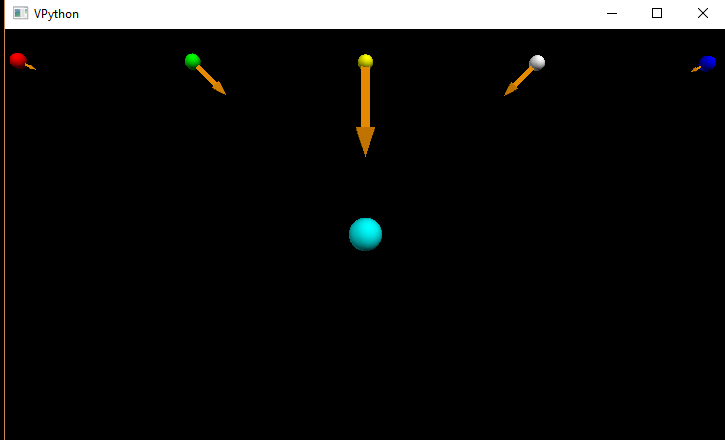
\includegraphics[height=5cm]{Untitled64.png}
\flushleft{}
\section{Problem 65}
Problem 65 has us make a spacecraft orbit the Earth, and vary the velocity and time steps to test the lower limits of our simulations and to find possible types of orbits.

\subsection{a)}
Part a instructs the user to vary velocity to find differnt types of orbits. At a low enough speed, my craft passes through the planet, and at high enough speed, it just travels in practically a straight line away from the planet. There is a range of speeds between $-10\leq$ $v_x$ $\leq-1$ where it travels in various tight ellipses and circles. I thought I would have found more hyperbolae and other various conic sections.

\subsection{b)}
Part b tells us to find a speed that renders an elliptical orbit. Through my playing around in part a, I found the most geometrically pleasing (to me anyway) elliptical orbit to be when $v_x = -10r_{Earth}$

\subsection{c)}
Adding arrows to the craft to show the velocity vector and force vector is illuminating, as it shows in orbital motion the two things are constantly perpendicular to one another. The arrows are shown in the figure below.
\centering
\\
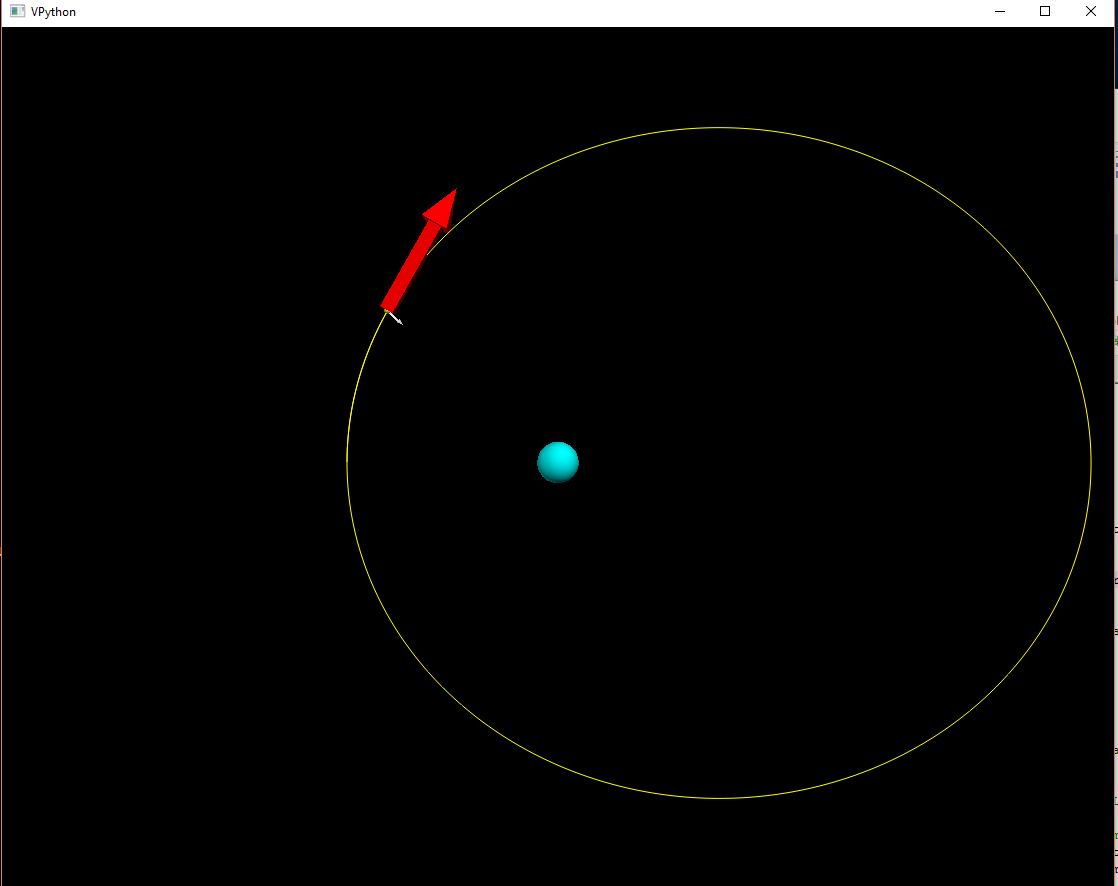
\includegraphics[height = 5cm]{Untitled65.png}
\flushleft{}

\subsection{d)}
Here we are instructed to find the speed that yeilds (yields? I should probably google that.) a circular orbit. I commented out the arrows on this one so the orbit would be more obvious, but I found the initial velocity $v_x$ to be equal to $-7r_{Earth}$ to get this sweet ring.
\centering
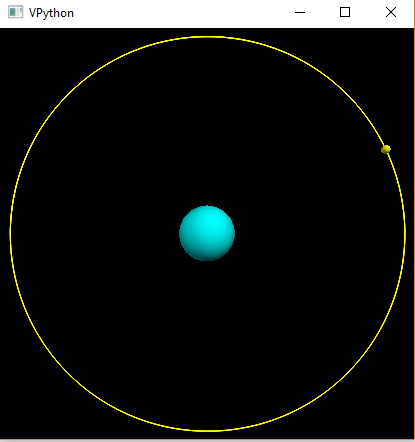
\includegraphics[height=5cm]{Untitled652.png}
\flushleft{}

\subsection{e)}
Our initial $\Delta t$ was 60, and I kept cranking it up and up until I noticed the orbit drifting. This happened when $\Delta t$ was approximately equal to 1000.

\section{Problem 66}
Here is another cool problem. It's basically the same as number 65, but with the added kink that we throw the moon into the mix. Somebody call Cixin Liu, cause we've got a Three Body Problem on our hands (Seriously though, that's a really good book)

\subsection{a)}

Find the initial speed such that the spacecraft orbits the Earth and the Moon. I've got a pretty stable orbit here at $3.4 \times 10^3$, though it looks like it will precess around the center of mass of the Earth-Moon system. In the program, the arrows work, but again, for clarity's sake, I commented them out for the picture.

\centering
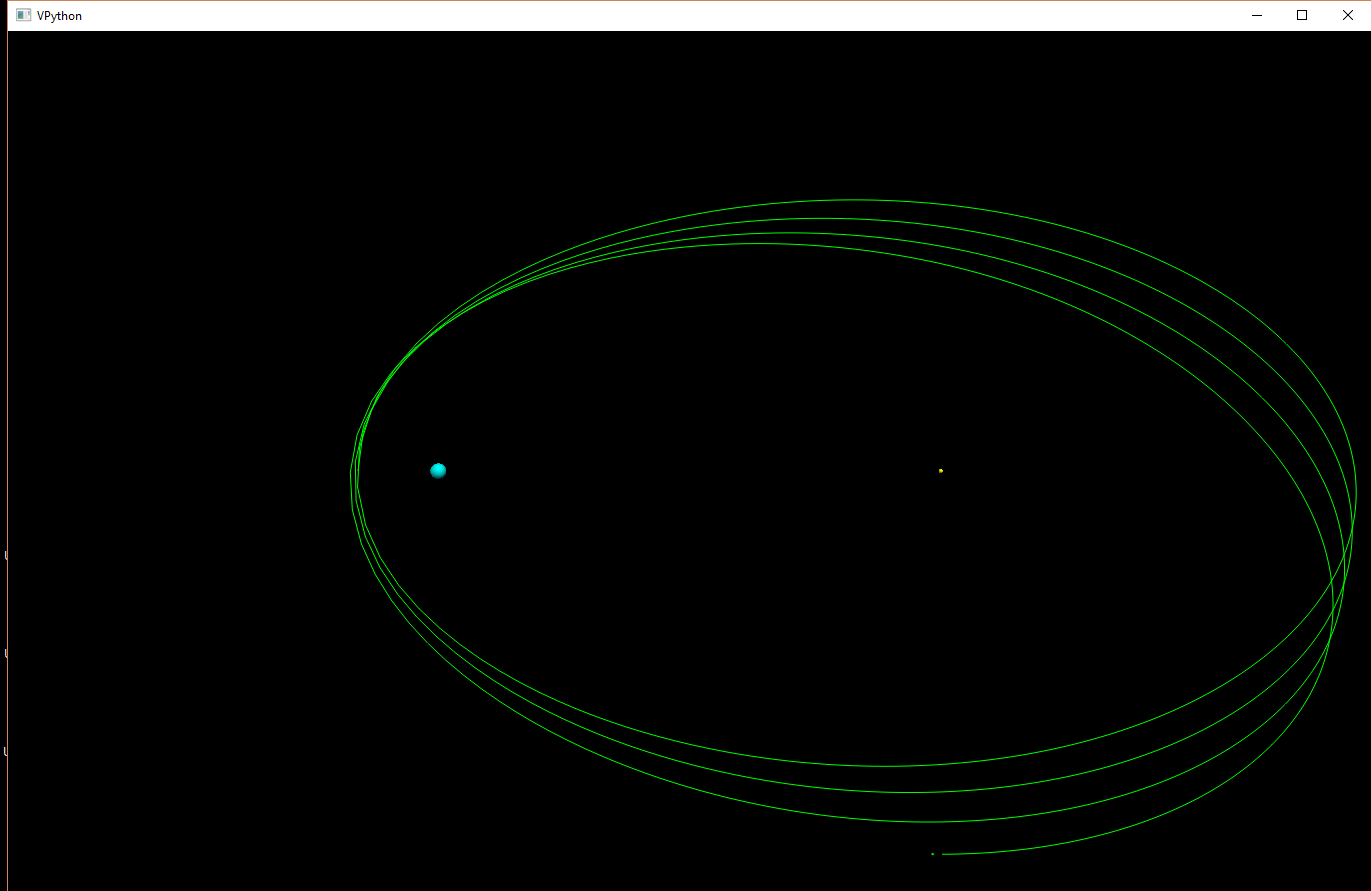
\includegraphics[height=5cm]{Untitled66a.png}
\flushleft{}

\subsection{b)}
For the life of me, I cannot get a figure eight orbit out of here. I've gotten some cool orbits where the ship interacts gravitationally with both bodies, and I've gotten it to make one halfway decent loop around both before being sent off into space, but I can't get a stable figure 8.

\subsection{c)}
This one's got some neat symmetry to it.
\\
\centering
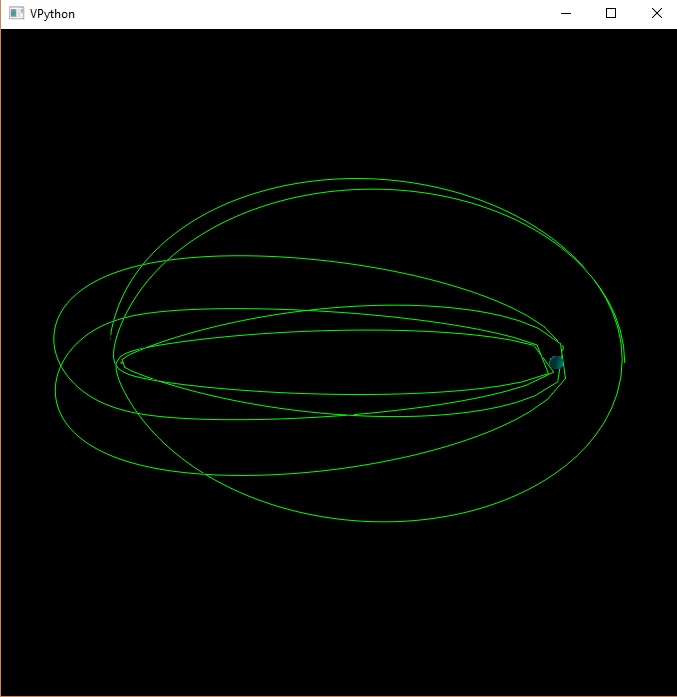
\includegraphics[height=5cm]{Untitled66b.png}
\end{document}
